% Масштабирование вычислений на суперкомпьютере.
\subsection{Масштабирование вычислений на суперкомпьютере}

\subsection{Organization of interprocess exchanges}

\begin{figure}[ht]
\centering
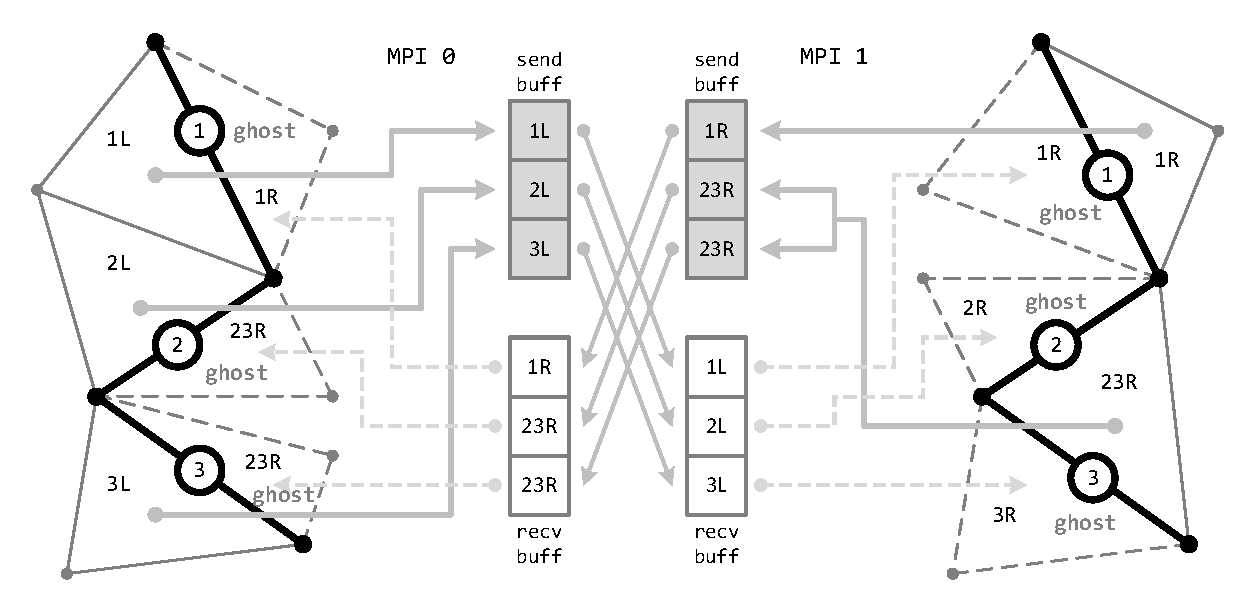
\includegraphics[width=1.0\textwidth]{pics/text_2_scaling/mpi.pdf}
\captionstyle{center}\caption{q}\label{fig:pic_classical_methods_multilayer}
\end{figure}

When performing calculations on a decomposed mesh, at each iteration of the computation, it is necessary to exchange data at each boundary between domains.
In our case, when performing the decomposition of the computational mesh, the boundary between two domains is represented by an arbitrary set of interdomain edges.
In this case, the boundary may be discontinuous, it may even consist of separate edges, therefore the order of interdomain edges in the sequence is not important when describing the boundary.

Fig.~\ref{fig:04-MPI} shows a scheme of organization of interprocess exchanges \cite{Rybakov_InnerRepresentation}.
Two domains (we will conventionally call them left and right), processed in MPI processes numbered 0 and 1, are separated by a boundary consisting of three edges.
In this case, there are three cells in the left domain that are adjacent to the considered boundary, in the right domain there are only two such cells (since cell 23R is adjacent to two edges of the boundary at once).
To organize interprocess communications in each domain, ghost cells are created for each edge of the considered boundary, which are involved in calculating flows through the edges.
At the same time, there is no need to recalculate physical values in ghost cells
All data for ghost cells is obtained using MPI exchanges from real cells of a neighboring domain.

To transfer data from the real border cells of the domain to the ghost cells of the neighboring domain, buffers for sending and receiving data are organized in each of the two neighboring domains.
The data exchange sequence is as follows (the diagram is shown in Fig.~\ref{fig:04-MPI}).
First, data from real boundary cells is written to the corresponding send buffers, then asynchronous commands \texttt{MPI\_Irecv} for receiving messages in the data receiving buffers are executed for all boundaries of the computational mesh.
After that, commands for asynchronous sending of data \texttt{MPI\_Isend} from the send buffers are also executed simultaneously for all boundaries of the computational mesh.
Next, it is necessary to wait for the completion of all asynchronous data exchanges using the \texttt{MPI\_Waitall} function.
The last step, completing the exchange of data between neighboring domains, is the transfer of the received physical values from the data receiving buffers to the corresponding ghost cells.

Note that some data duplication may occur when using ghost cells.
For example, in the presented diagram, cell 23R from the right domain corresponds at once to two ghost cells in the left domain.
These cells contain the same data.
This duplication of information is acceptable, since the data of the ghost cells is used only for reading to perform the calculation of flows across the domain boundary, therefore, in this case, there is no need to perform any synchronization of the same ghost cells.

\subsection{Efficiency of scaling supercomputer calculations}

To measure the scalability of computations on an unstructured surface computational mesh, a test surface of a streamlined three-dimensional body was used, containing about $ 2 \cdot 10^5 $ nodes and $ 4 \cdot 10^5 $ cells.
In the cells, calculations were performed related to modeling the flow of a liquid film, solving the heat balance equations on the surface, as well as remeshing and smoothing the surface.
To decompose the surface mesh, we used a simple hierarchical algorithm for halving domains, in which three coordinates of the center were taken as the features of the cells.
At the same time, as a result, the criterion for choosing a specific coordinate for dividing a domain was to minimize the length of the boundary between two domains (this approach allows dividing a domain along the longest direction).

\begin{table}[!h]
\label{tbl:supercomputers}
\setcaptionmargin{0mm}
\onelinecaptionsfalse
\captionstyle{flushleft}
\caption{The configurations of the segments of the MVS-10P OP supercomputer, on which the computation scaling measurements were taken.}
\bigskip
\begin{tabular}{|c|c|c|c|c|}
\hline
\parbox{3.5cm}{\textit{Family of\\Intel microprocessors}} & \parbox{4.0cm}{\textit{Number of\\processors/ cores /\\threads per node}} & \parbox{3.0cm}{\textit{Frequency of\\microprocessor}} & \parbox{3.0cm}{\textit{RAM\\per node}} & \parbox{2.0cm}{\textit{Supports\\AVX-512}} \\
\hline
Xeon Broadwell & 2 / 32 / 64 & 2.6 GHz & 128 GB & no \\
\hline
Xeon Phi KNL & 1 / 72 / 288 & 1.5 GHz & 96 GB & yes \\
\hline
Xeon Skylake & 2 / 36 / 72 & 3.0 GHz & 192 GB & yes \\
\hline
Xeon Cascade Lake & 2 / 48 / 96 & 3.0 GHz & 192 GB & yes \\
\hline
\end{tabular}
\label{tab:supercomputers}
\end{table}   

Homogeneous segments of the computing system of Joint Supercomputer Center of the Russian Academy of Sciences were used to measure the computational scalability \cite{JSCC_Supercomputers}.
In total, the calculations were carried out on four computational segments, the characteristics of the nodes of which are given in the table \ref{tab:supercomputers}.
In this table, it can be noted that all Intel \cite{Intel_SDM} microprocessors except Xeon Broadwell support the AVX-512 instruction set, which allows the use of special 512-bit vector registers for efficient code vectorization \cite{Savin_Vec}.
We should also highlight the computing nodes based on the Xeon Phi KNL microprocessor \cite{Jeffers_KNL}.
These microprocessors are distinguished by a huge number of computing cores, each of which is capable of executing up to 4 threads, which allows efficient parallelization of computational applications up to 288 threads on a single microprocessor.

\begin{figure}[ht]
\centering
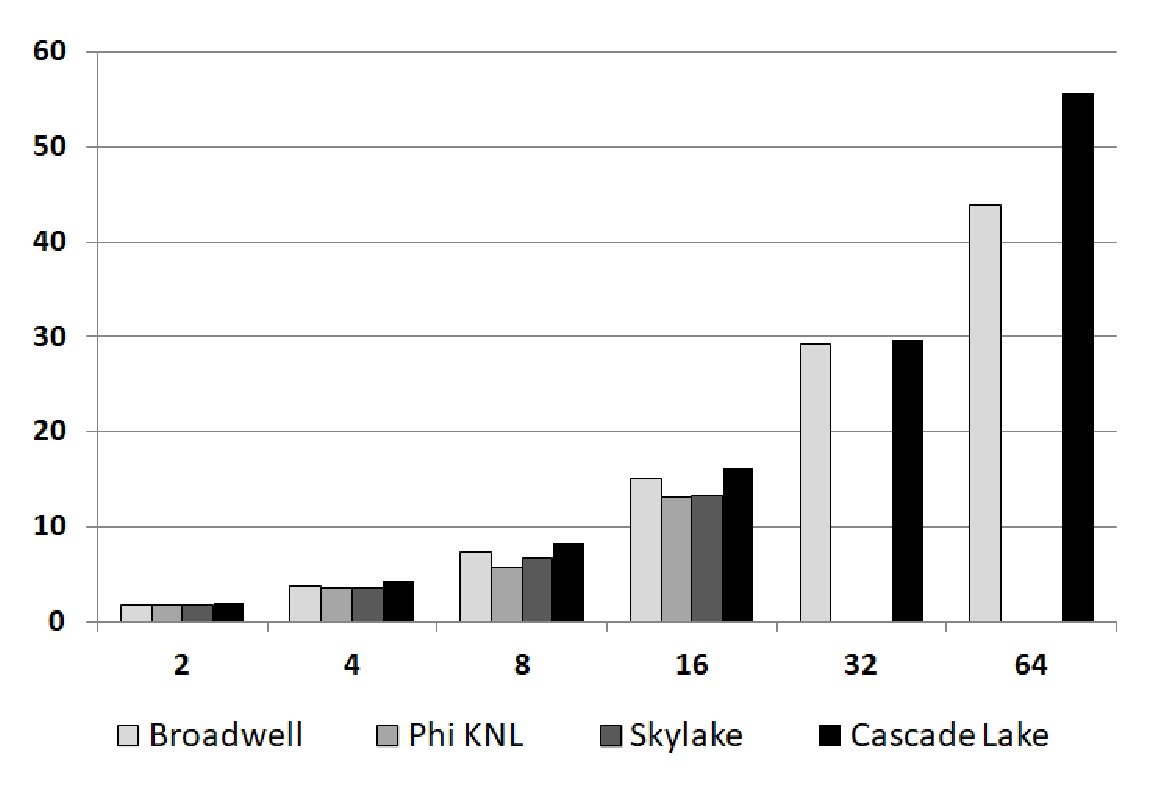
\includegraphics[width=0.8\textwidth]{pics/text_2_scaling/speedup.pdf}
\captionstyle{center}\caption{q}\label{fig:pic_classical_methods_multilayer}
\end{figure}

The main goal of the launches was to measure the strong scalability of computations with full parallelization within computational nodes using OpenMP.
That is, for all launches, the same surface was used (which was split over the required number of computational nodes), and all the threads available inside the computational nodes were also involved in the calculations.

When carrying out the calculations, the measurements were carried out independently for each computer system separately.
Let us give a description of the quantities measured in the calculation process for one specific computing system.
The time of the task execution on one computational node was used as the reference time: $ t(1) $.
We also measured the execution time of tasks for the number of computational nodes equal to a power of two (2, 4, 8, 16, 32, 64).
In this case, the acceleration on the number of nodes equal to $ i $ was considered the value of the value $ s(i) = \frac{t(1)}{t(i)} $.
Fig.~\ref{fig:speedup} shows diagrams of computation acceleration with an increase in the number of nodes for different computational systems.

In addition to calculating the direct speedup of code execution, the measurement of the scaling efficiency was performed.
In this case, the computational scaling efficiency is understood as the value $ e(i) = \frac{s(i)}{i} $.
The physical meaning of it is as follows.
We can assume that in the case of ideal parallelization of computations increasing the number of nodes by $ n $ times, the execution time decreases exactly by $ n $ times.
Thus, in the case of ideal parallelization, $ s (i) = i $, and $ e(i) = 1 $.
The efficiency of scaling computations is a convenient indicator of the quality of creating executable parallel code and comparing different computing systems with each other.
Note that super-linear scalability is quite possible (when the value of $ e(i) $ rises above one) \cite{Benderskiy_Scaling}, but this is more an exception than an expected effect.

\begin{figure}[ht]
\centering
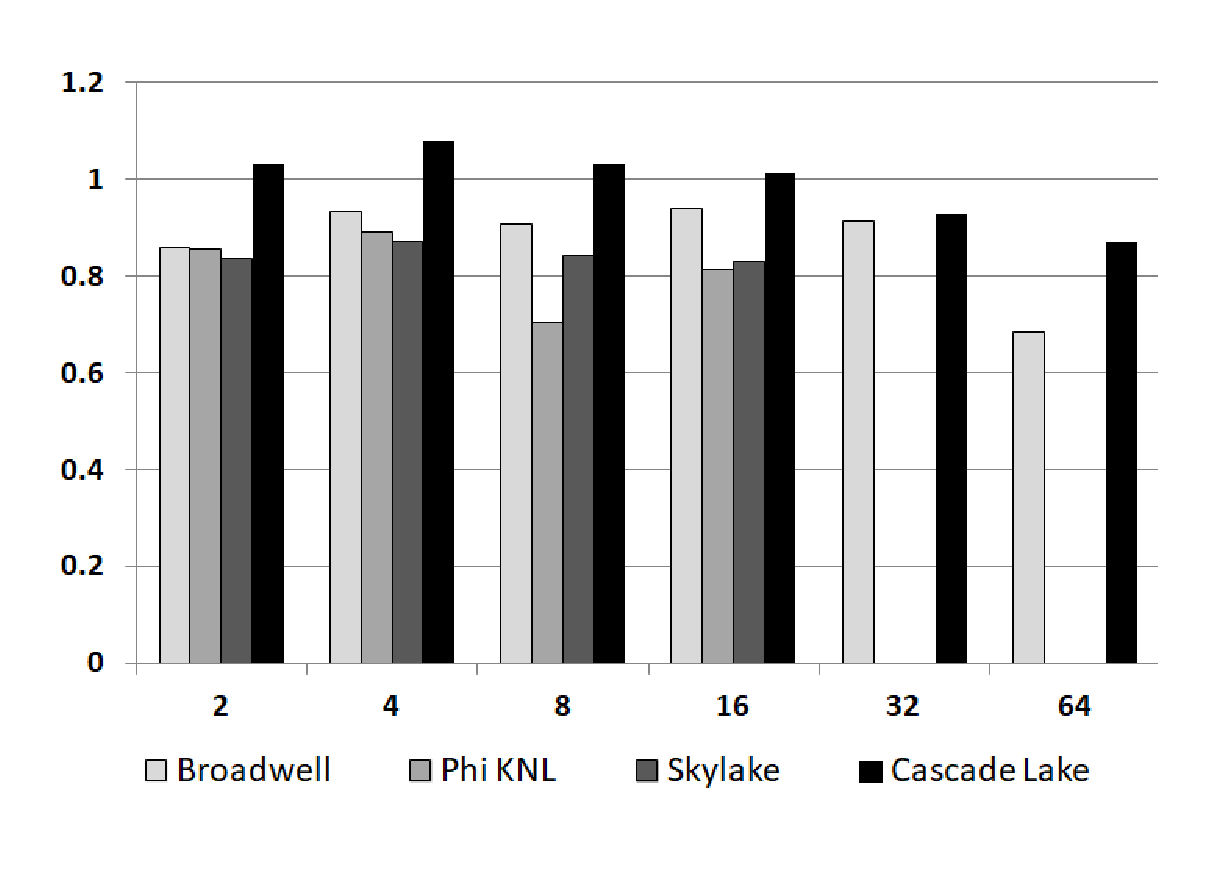
\includegraphics[width=0.8\textwidth]{pics/text_2_scaling/scaling.pdf}
\captionstyle{center}\caption{q}\label{fig:pic_classical_methods_multilayer}
\end{figure}

Fig.~\ref{fig:speedup} shows a diagram of the scaling efficiency of computations for various computational segments, depending on the number of computational nodes used.
It can be seen that for all computing systems, the scaling efficiency varies in the region of 0,8-0,9, although on some launch configurations there are dips even in the region of 0,7.
Launches with a low parallelization efficiency are usually associated with a spread in the processing time of MPI processes in their domains.
Despite the fact that the algorithm for decomposition of the computational mesh used in this article provided a uniform distribution of cells across domains, the processing time of a cell itself strongly depends on its physical properties and can differ significantly.
For this reason, balancing the computational load on different nodes is possible only in a dynamic mode \cite{Van_DynamicLoadBalance}, which was not done within the framework of this study.
We also note the high efficiency of scaling computations for compute nodes based on Xeon Cascade Lake microprocessors.
These processors are the most modern of all the equipment used in the described experiment.
